\documentclass{article}

\usepackage[ngerman]{babel}
\usepackage{datetime}
\usepackage[a4paper,top=2cm,bottom=2cm,left=3cm,right=3cm,marginparwidth=1.75cm]{geometry}
\usepackage{amsmath}
\usepackage{graphicx}
\usepackage{float} % For forcing the position of elements
\usepackage[colorlinks=true, allcolors=blue]{hyperref}
\usepackage{fancyhdr} % For custom headers and footers
\usepackage{titlesec}  % For automatic new page at sections
\usepackage{pdflscape}
\usepackage{longtable}
\usepackage{array}

% Set the Date Format
\newdateformat{myformat}{\THEDAY{ten }\monthname[\THEMONTH], \THEYEAR}

% Ensure a new page is started before every section
\newcommand{\sectionbreak}{\clearpage}
\newcommand{\thedate}{\today}

% Set up fancyhdr to customize the footer
\pagestyle{fancy}
\fancyhf{} % Clear default settings
\fancyfoot[C]{Pren Testat 1 Gruppe 16 - \thedate} % Add title and date to the center of the footer
\fancyfoot[R]{\thepage} % Page number on the right



\title{Pren Testat 1 Gruppe 16}
\author{Moritz Drillier \and Robin Venetz \and Benjamin Kuster \and Fabio Haueter \and Jonas Zimmermann \and Enya Senn}
\date{\thedate}

\begin{document}
\maketitle

\tableofcontents 


\section{Zeitplan}

\section{Teammitglieder}
\begin{figure}[H]
    \centering
    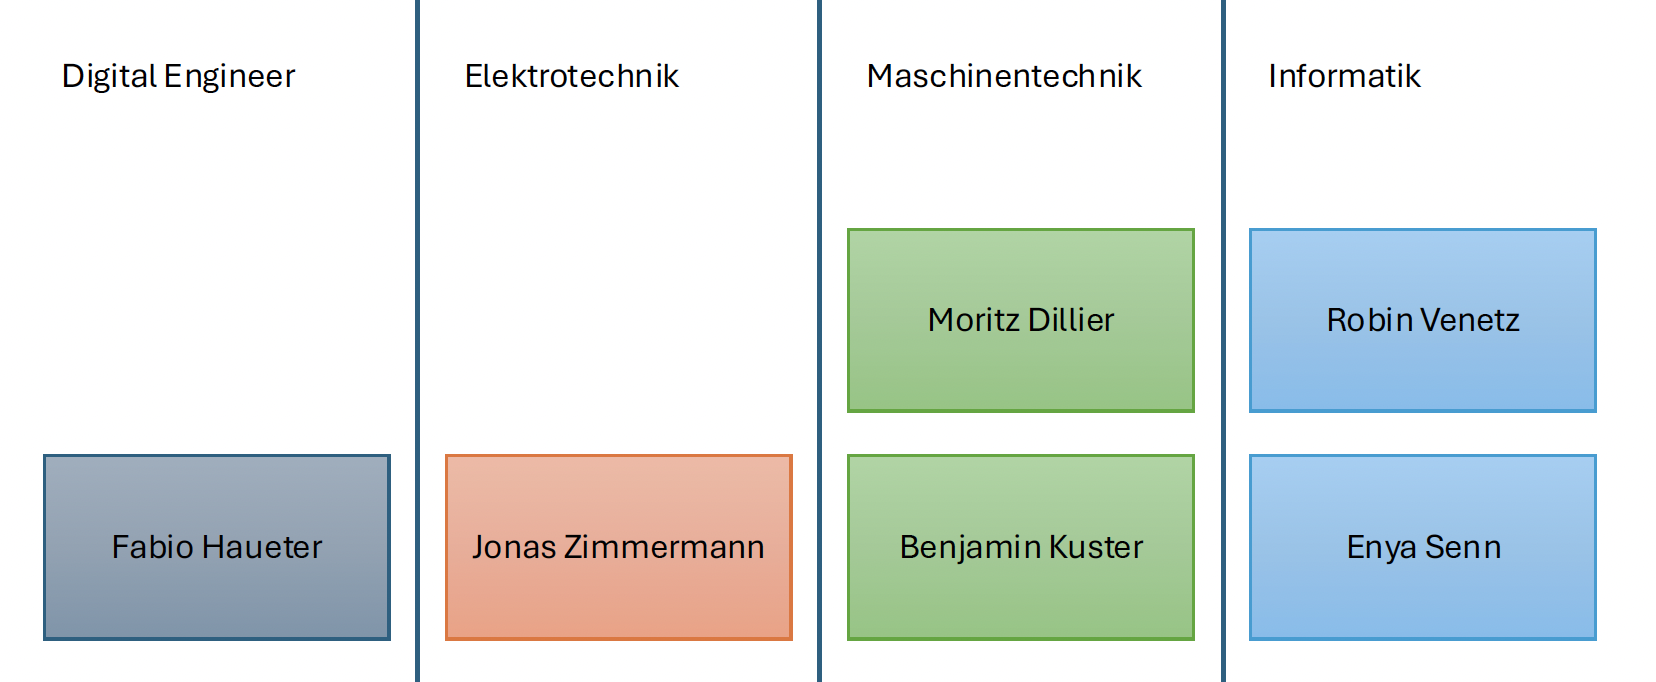
\includegraphics[width=0.8\linewidth]{Images/Pren_Gruppe.png}
    \caption{Teammitglieder}
    \label{fig:enter-label}
\end{figure}


\section{Aufgabenstellung}
In diesem Projekt wird ein autonomes Fahrzeug entwickelt, das sich in einem vorgegebenen Netzwerk von Wegpunkten (Nodes) und Kanten selbstständig orientieren und den optimalen Weg vom Start- zum Zielpunkt finden muss. Dabei müssen mehrere Herausforderungen bewältigt werden: Hindernisse auf der Strecke müssen erkannt, aktiv aufgehoben und an derselben Stelle wieder korrekt platziert werden. Zusätzlich dürfen gesperrte Wegpunkte (Nodes), die während des Fahrprozesses durch Markierungen gekennzeichnet werden, nicht befahren werden. Entfernte Kanten, die im Voraus nicht bekannt sind, werden vollständig aus dem Netz entfernt und sind für das Fahrzeug unsichtbar, was eine dynamische Anpassung der Routenplanung erfordert.

\hfill \break
Die Aufgabe erfordert eine präzise Pfadplanung, Echtzeit-Sensorverarbeitung sowie die Fähigkeit, auf unerwartete Änderungen im Netzwerk zu reagieren. Ziel ist es, dass das Fahrzeug den kürzesten und effizientesten Weg innerhalb eines komplexen, sich verändernden Streckennetzes unter Beachtung der vorgegebenen Regeln autonom bewältigt.

\begin{figure}[H]
    \centering
    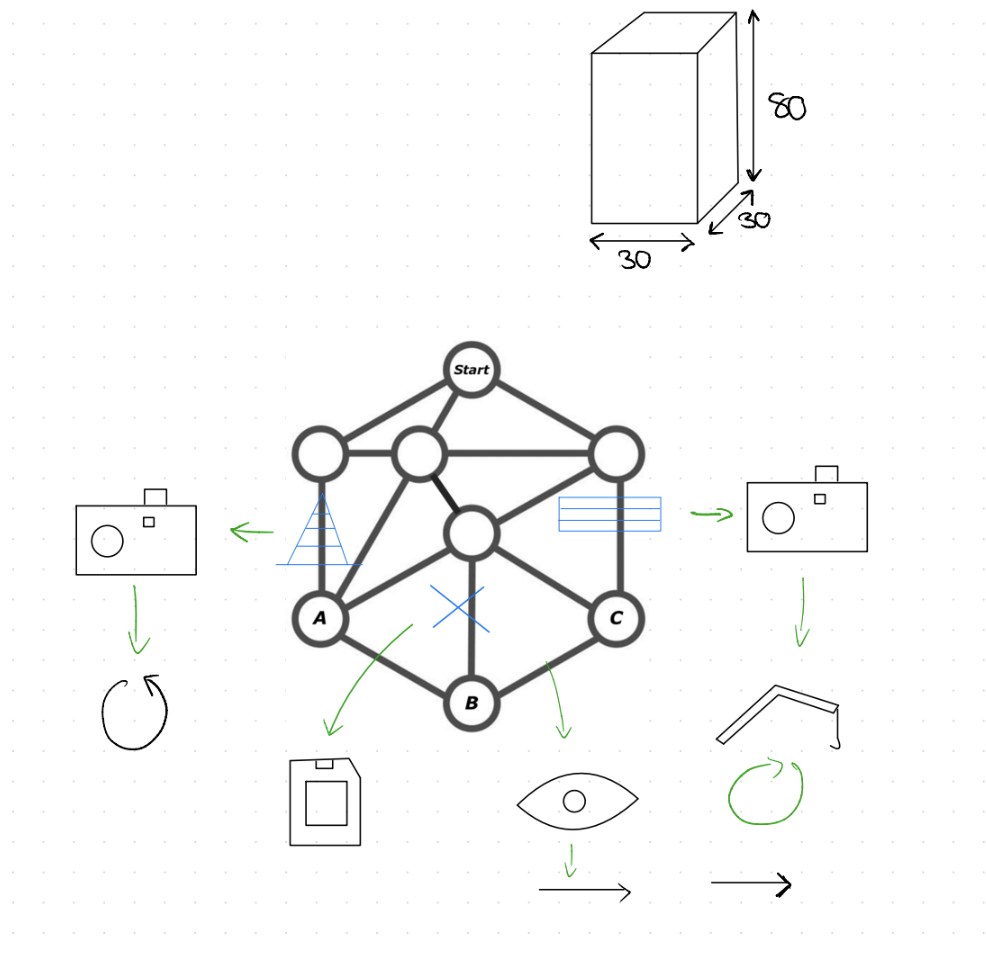
\includegraphics[width=0.6\linewidth]{Images/Pren_Skizze_Anforderungen.png}
    \caption{Aufgabenstellung Skizze}
    \label{fig:enter-label}
\end{figure}

\begin{landscape} % Begin landscape mode
\section{Anforderungsliste}
\begin{longtable}{>{\raggedright\arraybackslash}l>{\raggedright\arraybackslash}l>{\raggedright\arraybackslash}p{4cm}>{\raggedright\arraybackslash}p{15cm}>{\raggedright\arraybackslash}c}
    \textbf{Nr.} & \textbf{M/F/K} & \textbf{Thema/Frage} & \textbf{Erläuterung, Werte, Daten} & \textbf{Verantwortlich} \\
    \\
    \textbf{1} &  & \textbf{Gerät} & &   \\
    1.1 & F & Bauweise & Das Gerät muss eine Eigenkonstruktion sein. Einzelne Systemkomponenten, wie z.B. Servos,
    Motoren, Mikrocontrollerboard, Kamera u.a. dürfen zugekauft und eingesetzt werden. Es
    dürfen Software-Komponenten/-Services von Fremd-Herstellern verwendet werden. & E, I, M  \\ 
    1.2 & M & Geräteabmessung & l: 30 cm, b: 30 cm, h: 80 cm & M \\
    1.3 & M & Maximales Gewicht & 2kg & M \\
    1.4 & M & Kosten & Die Gesamtkosten in der ersten Phase dürfen nicht mehr als 200.- und insgesamt nicht mehr als 500.- sein. & \\
    1.5 & F & Nachhaltigkeit & Die Nachhaltigkeitsziele 9 sowie 12 müssen eingehalten werden & E, I, M \\
    1.6 & F & Wahlschalter & Das Fahrzeug muss einen Wahlschalter besitzen, mit welchem man zwischen den Zielen A, B und C wählen kann. & E, I \\
    1.7 & F & Not-Aus & Das Fahrzeug muss einen immer zugänglichen Not-Aus Schalter besitzen, welcher der mechanisch-dynamische Prozess
    jederzeit sofort unterbricht. & E, I, M \\
    1.8 & M & Aufbauzeit & Das Fahrzeug muss innerhalb von 1 Minute auf der Markierung platziert, aufgebaut und betriebsbereit sein. & \\
    \\
    \textbf{2} &  & \textbf{Fahrt/Ablauf} & &   \\
    2.1 & F & Startbefehl & Startknopf / Taster / Schalter & E, I \\
    2.2 & M & Autonomes Fahren & Beim Befahren der Linie muss immer ein Teil des Fahrzeugs auf der Linie verbleiben (ca. 20mm breite Linie) & E, I \\
    2.3 & M & Wegpunkte & Es gibt aufgeklebte Wegpunkte, von denen mind. 2 abgefahren werden müssen. & I \\
    2.4 & M & Fahrzeit & Die Fahrzeit darf maximal 4 Minuten betragen. & \\
    2.5 & F & Hindernisse & Hindernisse müssen erkannt, aufgehoben und an die selbe Stelle gestellt werden (20mm Toleranz). (Schneepflug/fortschieben nicht zulässig). & E, I, M \\
    2.6 & F & Sperrungen & Sperrungen müssen erkannt werden und dürfen nicht bewegt werden. & E, M, I \\
    2.7 & F & Entfernte Routen & Entfernte Routen müssen erkannt und können nicht genutzt werden. & E, I \\
    2.8 & M & Zielposition & Das Fahrzeug muss in einem Radius von 15 cm um den gewählten Zielpunkt zum Stehen kommen. & E, I \\
    2.9 & M & Erreichen des Endes & Das Erreichen der Zielposition muss visuell oder akustisch signalisiert werden. & E, I \\
    \\
    \textbf{3} & & \textbf{Randbedingungen} \\
    3.1 & F & Wegpunkte & Vollkreis, weiss, D = 7 - 12 cm & Doz. \\
    3.2 & F & Verbindungslinien Länge & 0.5 - 2 m & Doz. \\
    3.3 & F & Verbindungslinien Breite & 20 mm +/- 5 mm & Doz. \\
    \\
    3.4 & F & Abmessung Hindernis & 135 x 38 x 60 mm, je +/- 15 mm & Doz. \\
    3.5 & F & Gewicht Hindernis & ca. 200 g & Doz. \\
    3.6 & F & Untergrund & Als Untergrund dient der Boden im Foyer vor der Mensa & Doz. \\
    \\
    \textbf{4} & & \textbf{Simulation} \\
    4.1 & M & Art & Kein physischer Prototyp & I \\

\end{longtable}
\end{landscape} % End landscape mode

\begin{landscape} % Begin landscape mode
	\section{Technische Recherche}
	\begin{longtable}{>{\raggedright\arraybackslash}p{3cm}>{\raggedright\arraybackslash}p{3cm}>{\raggedright\arraybackslash}p{5cm}>{\raggedright\arraybackslash}p{5cm}>{\raggedright\arraybackslash}p{1cm}>{\raggedright\arraybackslash}p{7cm}}		
		\textbf{Funktion}               & \textbf{Möglichkeiten} & \textbf{Vorteile}                                                                                & \textbf{Nachteile}                                                             & \textbf{Quelle}                                                                                              & \textbf{Beschreibung}                                                                                                                                                                                                                                                                                                                                                                                                                                                                     \\
		\textbf{Linie folgen}           &                         &                                                                                                  &                                                                                &                                                                                                              &                                                                                                                                                                                                                                                                                                                                                                                                                                                                                           \\
		Linie erkennen                  & Infrarotsensor          & Einfache erkennung der Linie                                                                     & Durch Lichteinstrahlung beeinflusst                                            & \href{https://www.futurelearn.com/info/courses/robotics-with-raspberry-pi/0/steps/75899}{Link}               & Der Sensor sendet IR Licht aus und misst, wie viel Licht reflektiert wird.                                                                                                                                                                                                                                                                                                                                                                                                                \\
		                                & Kamera                  & Flexibler / kann auch für Objekterkennung genutzt werden                                        & Komplizierter als ein Infrarotsensor. Reflektierendes Licht kann beeinflussen. & \href{https://www.instructables.com/Line-Following-Robot-Using-Smartphones-Camera/}{Link}                    & Erkennung der Linie durch Farberkennung auf Bildern                                                                                                                                                                                                                                                                                                                                                                                                                                       \\
		                                & Farbsensor              & Kann mehrere Farben einfach erkennen (falls Linie bunt)                                          & Empfindlich gegen Lichteinstrahlung                                            & \href{https://robotics.stackexchange.com/questions/2491/how-are-color-sensors-used-for-line-following}{Link} & Erkennung der Linie durch Erkennung der Farbe und des Farbkontrasts                                                                                                                                                                                                                                                                                                                                                                                                                       \\
		Auf der Linie\break bleiben     & 1 Sensor                & Geringe Kosten.                                                                                  & Ort auf der Linie nicht bekannt                                                &                                                                                                              & Der Linie wird mit einem Sensor gefolgt. Wenn sie verlassen wird, werden Anpassungen vorgenommen                                                                                                                                                                                                                                                                                                                                                                                          \\
		                                & 2+ Sensoren             & Immer bekannt, wo/wie man sich auf der Linie befindet                                            & Höhere Kosten                                                                 & \href{https://robotics.stackexchange.com/questions/2491/how-are-color-sensors-used-for-line-following}{Link} & Der Linie wird mit einem Sensor gefolgt. Wenn sie verlassen wird, werden Anpassungen vorgenommen                                                                                                                                                                                                                                                                                                                                                                                          \\
		                                & Kamera                  & Nur eine Kamera nötig                                                                           & Komplexität                                                                   &                                                                                                              & Mit einer Kamera kann der Verlauf und der Position erkannt werden und Anpassungen an der Richtung vorgenommen werden                                                                                                                                                                                                                                                                                                                                                                      \\
										
		\textbf{Hindernisse}            &                         &                                                                                                  &                                                                                &                                                                                                              &                                                                                                                                                                                                                                                                                                                                                                                                                                                                                           \\
		Identifikation& Bilderkennung
		&  Kann beide Objekte erkennen und differenzieren& Hohe Rechenleistung benötigt& \href{https://www.delftstack.com/de/howto/python/color-detection-opencv/}{Link}& Mittels Bilderkennung (OpenCV) werden die Hindernisse erkannt
		\\
		                                & Farbsensor              & Einfache differenzierung der Hindernisse falls unterschiedliche Farbe                            & Ähnliche Farben können schwierig zu unterscheiden sein                       & \href{https://www.electronicshub.org/raspberry-pi-color-sensor-tutorial/}{Link}                              & Erkennung der Farben. Evenutell mit zwei Unterschiedlich hohen Farbsensoren                                                                                                                                                                                                                                                                                                                                                                                                               \\
		Distanzmessung                  & Ultraschallsensor       & Billig, einfache Implementation/Integration                                                      & Limitierte Distanz und Genauigkeit                                             & \href{https://www.geeksforgeeks.org/distance-measurement-using-ultrasonic-sensor-and-arduino/}{Link}         & Messung der Distanz zum Objekt mittels Ultraschallwellen                                                                                                                                                                                                                                                                                                                                                                                                                                  
		\\
		                                & LIDAR                   & Genaue Karte der Umgebung kann erstellt werden                                                   & Preis                                                                          & \href{https://de.wikipedia.org/wiki/Lidar}{Link}                                                             & Funktioniert ähnlich wie ein Ultraschallsensor. Misst Distanzen jedoch mittels Laserstrahlen                                                                                                                                                                                                                                                                                                                                                                                             \\
		\textbf{Simulation}             &                         &                                                                                                  &                                                                                &                                                                                                              &                                                                                                                                                                                                                                                                                                                                                                                                                                                                                           \\
		Simulation der Funkionalitäten & Unity                   & In C\# programmierbar, Funktionalität kann bereits getestet werden                              &                                                                                & \href{https://unity.com/de}{Link}                                                                            & Simuluation des Fahrzeuges in der GameEngine Unity. Es können Kameras und Sensoren simuliert werden.Auch können Lichteinflüsse simuliert werden.                                                                                                                                                                                                                                                                                                                                       
		\\
		                                & Website                 & Einfach erreichbar, schnelles Prototyping, Cross, Platform                                       & Limitierte Performance, nur in JS programmierbar                               & \href{https://threejs.org/}{Link}                                                                            & Mittels WebGL und einer Library wie three.js können 3D umgebungen im Webbrowser simuliert werden.                                                                                                                                                                                                                                                                                                                                                                                        
		\\
		                                & Panda3D?                &                                                                                                  &                                                                                &                                                                                                              &                                                                                                                                                                                                                                                                                                                                                                                                                                                                                           \\
		                                & UnrealEngine            & Programmierbar, Logik kann bereits getestet werden                                               & Wenig Kenntnisse in C++                                                        & \href{https://www.unrealengine.com/de}{Link}                                                                 & Simuluation des Fahrzeuges in der GameEngine UnrealEngine. Es können Kameras und Sensoren simuliert werden.Auch können Lichteinflüsse simuliert werden.                                                                                                                                                                                                                                                                                                                                \\
		\textbf{Weg finden}             &                         &                                                                                                  &                                                                                &                                                                                                              &                                                                                                                                                                                                                                                                                                                                                                                                                                                                                           \\
		Algorithmus der Wegfindung      & dijkstra algorithm      & Garantiert den kürzesten Weg in einem statischen Netzwerk.                                      &                                                                                & \href{https://www.geeksforgeeks.org/dijkstras-shortest-path-algorithm-greedy-algo-7/}{Link}                  & Er könnte verwendet werden, um die kürzeste Strecke vom Startpunkt zum Ziel zu bestimmen, basierend auf dem Wege-Netzwerk. Bei Hindernissen oder gesperrten Knoten könnte der Algorithmus dynamisch die Route anpassen, indem er die entsprechenden Knoten ausschließt.                                                                                                                                                                                                               \\
		
		                                & Allstar Algorithmus     & Effizienter als Dijkstra durch die Verwendung einer Heuristik, die den Zielpunkt berücksichtigt & Die Wahl der Heuristik beeinflusst die Effizienz stark.                        & \href{https://www.simplilearn.com/tutorials/artificial-intelligence-tutorial/a-star-algorithm }{Link}        & Erweiterung des Dijkstra-Algorithmus und berücksichtigt zusätzlich eine Heuristik, um effizienter zu sein. Dieser Algorithmus könnte verwendet werden, um den optimalen Pfad zu berechnen, während er Hindernisse und Sperren berücksichtigt.                                                                                                                                                                                                                                        \\
		                                &                         &                                                                                                  &                                                                                &                                                                                                              &                                                                                                                                                                                                                                                                                                                                                                                                                                                                                           \\
		                                &                         &                                                                                                  &                                                                                &                                                                                                              &                                                                                                                                                                                                                                                                                                                                                                                                                                                                                           \\
		\textbf{Programiersprache}      &                         &                                                                                                  &                                                                                &                                                                                                              &                                                                                                                                                                                                                                                                                                                                                                                                                                                                                           \\
		Programierung des Raspberry PI  & Python                  & Weit verbreitet, portable, viele Libraries, häufig für ML verwendet                            & Permformance limitationen                                                      & \href{https://threejs.org/}{Link}                                                                            & Python ist die bevorzugte Sprache für ML auf dem Raspberry Pi, da es eine riesige Auswahl an ML-Bibliotheken bietet. Zudem hat es eine einfache Syntax und eine starke Community-Unterstützung. Es ist auch leicht, Python-Programme mit den GPIO-Pins zu verbinden, was den Einsatz von Sensoren und Aktoren in ML-Projekten erleichtert.                                                                                                                                              
		\\
		                                & C\#                     & Bereits bekannt, kann in Unity getestet werden, Cross-Platform, Performance                      & Wenig Libraries für GPIO, noch nicht sehr lange unterstützt                  & \href{https://learn.microsoft.com/de-de/dotnet/iot/deployment}{Link}                                         & C\# kann über .NET oder Mono auf dem Raspberry Pi verwendet werden. Es gibt ML-Frameworks wie ML.NET, die in C\# für ML-Aufgaben auf dem Raspberry Pi genutzt werden können. C\# bietet eine objektorientierte Struktur und ist ideal für komplexere, skalierbare ML-Anwendungen. Die Performance ist besser als bei Python, aber der Zugriff auf GPIO und Hardware für ML-Anwendungen ist eingeschränkter. GPIO: https://learn.microsoft.com/en-us/dotnet/iot/tutorials/gpio-input 
		\\
		                                & Java                    & Protable                                                                                         & Weniger verrbreitet, weniger Libraries für H7                                 & \href{https://threejs.org/}{Link}                                                                            & C++ wird oft für ML auf Systemen mit beschränkten Ressourcen wie dem Raspberry Pi verwendet, insbesondere wenn Leistung entscheidend ist. Bibliotheken wie TensorFlow Lite und OpenCV sind in C++ verfügbar und können für ML-Aufgaben eingesetzt werden. C++ bietet die beste Leistung und direkte Hardwarezugriffe, was es für komplexe ML-Anwendungen und Echtzeit-Prozesse ideal macht.                                                                                         
		\\
		                                & C++                     & Performant, Low-level access, viele Libraries                                                    & Komplex, eigenes Memory-Management, wenig Kenntnisse                           & \href{https://threejs.org/}{Link}                                                                            & Java ist über OpenJDK auf dem Raspberry Pi verfügbar und kann für Machine Learning eingesetzt werden, etwa mit Bibliotheken wie Deeplearning4j. Es bietet plattformunabhängige Unterstützung und eignet sich gut für vernetzte Anwendungen, die auf ML-Modelle zugreifen müssen. Die Performance ist besser als bei Python, aber schwächer als bei C++. Der Hardwarezugriff über GPIO ist jedoch eingeschränkt.                                                                 \\
				                                
	\end{longtable}
\end{landscape} % End landscape mode

\listoffigures % Abbildungsverzeichnis
\listoftables % Tabellenverzeichnis

\end{document}
